\subsection{Throw Detection Mechanism}
\label{subsec:throw_detection_mechanism}

To reliably detect a throw, a simple image change detection algorithm is implemented.
It requires a repeated difference computation and therefore a circular buffer is used.

This section explains the employed algorithm, its implementation and the saving of the images.

% \subsubsection{Image Change Detection Algorithm}
% \subsubsection{Throw Detection Algorithm}
\subsubsection{Employed Algorithm}
\label{subsubsec:algorithm}
% \todo[inline]{No citations?! Or OpenCV?! Or Baumer?!}

% image change detection algorithm vs throw detection / throw detection mechanism / throw detection algorithm => throw detection employs icda

% Goal of the throw detection is to extract the valid frames of a throw from the continous data stream
  % valid frames have object on them, invalid frames are empty (background)
% real-time
% serial process, 200 fps => >5 ms to process each frame
% not a lot of time for a complex (fancy) algorithm => simplest one possible is used
  % for the throw detection algorithm a simple image change detection algorithm is used

% Algo: computation of the difference and comparison to a threshold to detect changes in the picture

% what this sections describes

% Due to the in section {} mentioned bandwidth limitations of the U3V interface the raw bayer is processed
  % conversion to BGR8 takes too long! => use raw bayer for the detection
% Saving images takes time + unnecessary => saving at the end!
  % see section \ref

% buffers

% frame_id (FID) to keep track of ...
% uses 2 flags and 2 "pointers" to the buffer

% compared against threshold (if mean_diff < threshold, considered to be no change [equal sign])

% throw begin and throw end, what happens

% Why are the last two frames are not valid?
  % only possible to detect the end when there is no change any longer

The goal of the throw detection is to extract valid frames of a throw --- with objects on them --- from the continous data stream of the camera.
Therefore, the throw detection needs to work in real time.
At a frame rate of \SI{200}{fps}, there is $<\SI{5}{ms}$ to process a single frame (without the use of parallel computing).
Due to this time constraint, a simple image change detection algorithm is employed.

\paragraph{Image Change Detection Algorithm}
\vspace{-20pt}
\begin{enumerate}
  \item Compute the absolute difference between the current and the last frame
  \item Compute the average among all the pixels of the difference
  \item Compare the mean difference against a threshold value
\end{enumerate}

This section describes how the throw detection works.
The complete listing of the throw detection can be found in appendix \ref{app:throw_detection}.
The implementation of the image change detection is described in section \ref{subsubsec:image_change_detection}.
Furthermore, the way the threshold value is obtained is documented in section \ref{subsubsec:threshold}.

Due to the bandwidth limitations of the U3V interface mentioned in section \ref{subsubsec:usb3_vision_interface}, the received images are in the raw Bayer pixel format.
A conversion from the Baumer \texttt{BayerRG8} to \texttt{BGR8} takes too long an therefore the raw frames are processed.
Moreover, the valid images are only saved on the hard disk at the end of a throw, as this also takes a lot of time (see section \ref{subsubsec:saving_images}).

For the above reasons, two image buffers are used.
The received images are stored in Baumer \texttt{BGAPI2::Buffer} objects.
To save the images later on, a circular buffer for OpenCV matrices (\texttt{cv::Mat}) is used.
This is documented in section \ref{subsubsec:buffers}.
The size of those image buffers (\texttt{BS}) determines the max. amount of valid frames $N_\text{max}$ that can be captured.

To keep track of the present and past frames, a frame id (\texttt{FID}) is utilized.
Furthermore, two flags are used to mark the beginning and the end of a throw.

Whenever the mean difference between two consecutive frames is greater than or equal to the threshold, they are considered to be different ($\ne$).
Otherwise, the two frames are considered to be equal ($=$).

Once two consecutive frames are different, the flag \texttt{throw\_bgn} is set to \texttt{true} and the current \texttt{FID} is saved in \texttt{throw\_bgn\_idx}.
The current and all subsequent frames --- except for the last two --- belong to the detected throw until two consecutive frames are no longer different.
In this case, the flag \texttt{throw\_end} is set to \texttt{true} and the current \texttt{FID} is saved in \texttt{throw\_end\_idx}.

The last two frames are not valid due to the way the throw detection works.
The first invalid frame occurs when the object leaves the image, as this is still a change in the image and thus not detected.
The second invalid frame results from the fact that the following images are only now the same and therefore the current \texttt{FID} is saved.

Figure \ref{subfig:algorithm_general_case} shows the general case of the just described throw detection.
As already mentioned, the max. amount of valid frames $N_\text{max}$ depends on the image buffer size (\texttt{BS}).
To properly detected a throw, the amount of valid frames $N$ must meet the condition
\[
  N \in \{1..(\text{BS}-2)\}.
\]
In the current implementation, an image buffer size of \SI{1000}{} is used and therefore $N_\text{max} = \SI{998}{frames}$.
An example of three valid frames ($N = 3$) is shown in figure \ref{subfig:algorithm_example_3}.

\begin{figure}[h]
  \centering
  \begin{subfigure}[b]{\textwidth}
    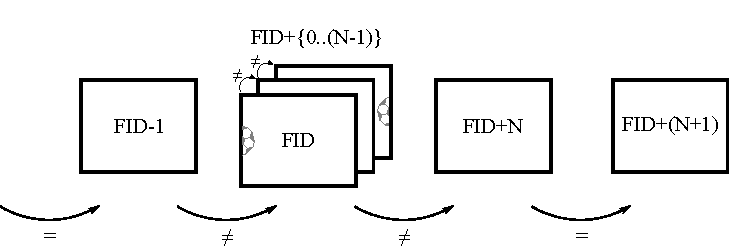
\includegraphics[scale=0.85]{algorithm}
    \caption{General case with $N \in \{1..(\text{BS}-2)\}$}
    \label{subfig:algorithm_general_case}
  \end{subfigure}
  \begin{subfigure}[b]{\textwidth}
    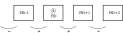
\includegraphics[scale=0.85]{algorithm_ex_1}
    \caption{Example of $N_\text{min} = 1$}
    \label{subfig:algorithm_example_1}
  \end{subfigure}
  \begin{subfigure}[b]{\textwidth}
    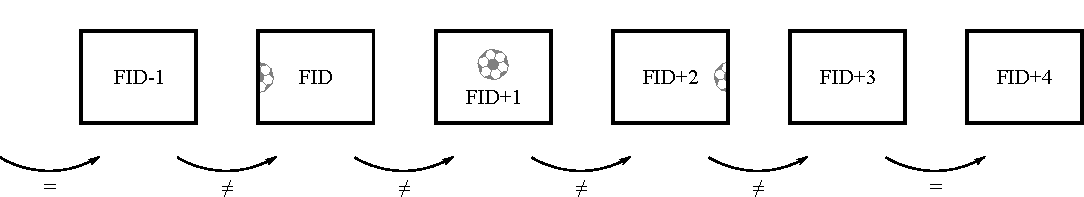
\includegraphics[scale=0.85]{algorithm_ex_3}
    \caption{Example of three valid frames ($N = 3$)}
    \label{subfig:algorithm_example_3}
  \end{subfigure}
  \caption{Illustration of the throw detection}
  \label{fig:throw_detection}
\end{figure}

\subsubsection{Image Buffers}
\label{subsubsec:buffers}
\todo[inline]{Citations}

Two different buffers with the same buffer size (\texttt{BS}) are used.
A Baumer image buffer to receive the images and an OpenCV matrix cirucular buffer to manipulate and save the images.

\paragraph{Baumer Image Buffer}
The received images are stored in Baumer \texttt{BGAPI2::Buffer} objects.
These are instantiated with the default constructor \texttt{BGAPI2::Buffer::Buffer()}, which allocates enough memory for the maximum payload of the camera.
In this case the maximum payload of the industrial camera is determined by the \texttt{BGR8} pixel format.
As a result of this, the memory utilization for the Baumer \texttt{BayerRG8} pixel format is only \SI{33}{\percent}.
Table \ref{tab:buffer_memory_utilization} shows the required memory as well as the memory utilization for the two pixel formats \texttt{BayerRG8} and \texttt{BGR8}.

It is possible to get \SI{100}{\percent} memory utilization with the Baumer \texttt{BayerRG8} pixel format.
The necessary memory for the specific payload size can be allocated manually and then passed to the constructor.
However, the software is not designed to run on an embedded system but on a computer.
Every modern computer should have the required resources to run the program.
% https://www.baumer.com/ch/en/product-overview/industrial-cameras-image-processing/software/baumer-gapi-sdk/c/14174

\begin{table}[h]
  \caption{Baumer image buffer memory utilization for the pixel formats \texttt{BayerRG8} and \texttt{BGR8}}
  \label{tab:buffer_memory_utilization}
  \centering
  \begin{tabular}{lll}
    \toprule
     & \textbf{\texttt{BayerRG8}} & \textbf{\texttt{BGR8}} \\
    \midrule
    \textbf{Bytes per pixel} & \SI{1}{B} & \SI{3}{B} \\
    \textbf{Pixel count} & \SI{1310720}{px} & \SI{1310720}{px} \\
    \textbf{Pixel bytes} & \SI{1310720}{B} & \SI{3932160}{B} \\
    \textbf{Buffer size} & \SI{3932160}{B} & \SI{3932160}{B} \\
    \textbf{Utilization} & \SI{33}{\percent} & \SI{100}{\percent} \\
    \bottomrule
  \end{tabular}
\end{table}

% --------------------------------
\paragraph{OpenCV Circular Buffer}
OpenCV matrix \texttt{cv::Mat} objects are used to perform the necessary image manipulations (see section \ref{subsubsec:image_change_detection}).
The data pointer of the Baumer image buffer is used to create an OpenCV matrix as shown in appendix \ref{app:throw_detection} on line \ref{lst:ln:buffer}.
This way, the OpenCV matrix does not allocate memory for the matrix data and uses the specified data.
The reasons for only creating such a shallow copy are efficiency and memory space.
% https://docs.opencv.org/4.1.1/d3/d63/classcv_1_1Mat.html#a51615ebf17a64c968df0bf49b4de6a3a
% https://www.baumer.com/ch/en/service-support/know-how/technical-information-industrial-cameras/baumer-gapi-and-opencv/a/baumer-gapi-and-opencv

In order to be able to save the images later, past OpenCV matrices must be available.
For this reason, an OpenCV matrix circular buffer is used to keep track of them.
The structure of the circular buffer is shown in figure \ref{fig:circular_buffer}.
The circular buffer size (\texttt{BS}) is the same as the Baumer image buffer size.
The elements of the circular buffer can be accessed through an index $I$.
This index $I$ depends on the frame id (\texttt{FID}) and is calculated using equation \ref{eq:indexing}.

\begin{equation}
  I \equiv \text{FID} \pmod{\text{BS}}
  \label{eq:indexing}
\end{equation}

\begin{figure}[h]
  \centering
  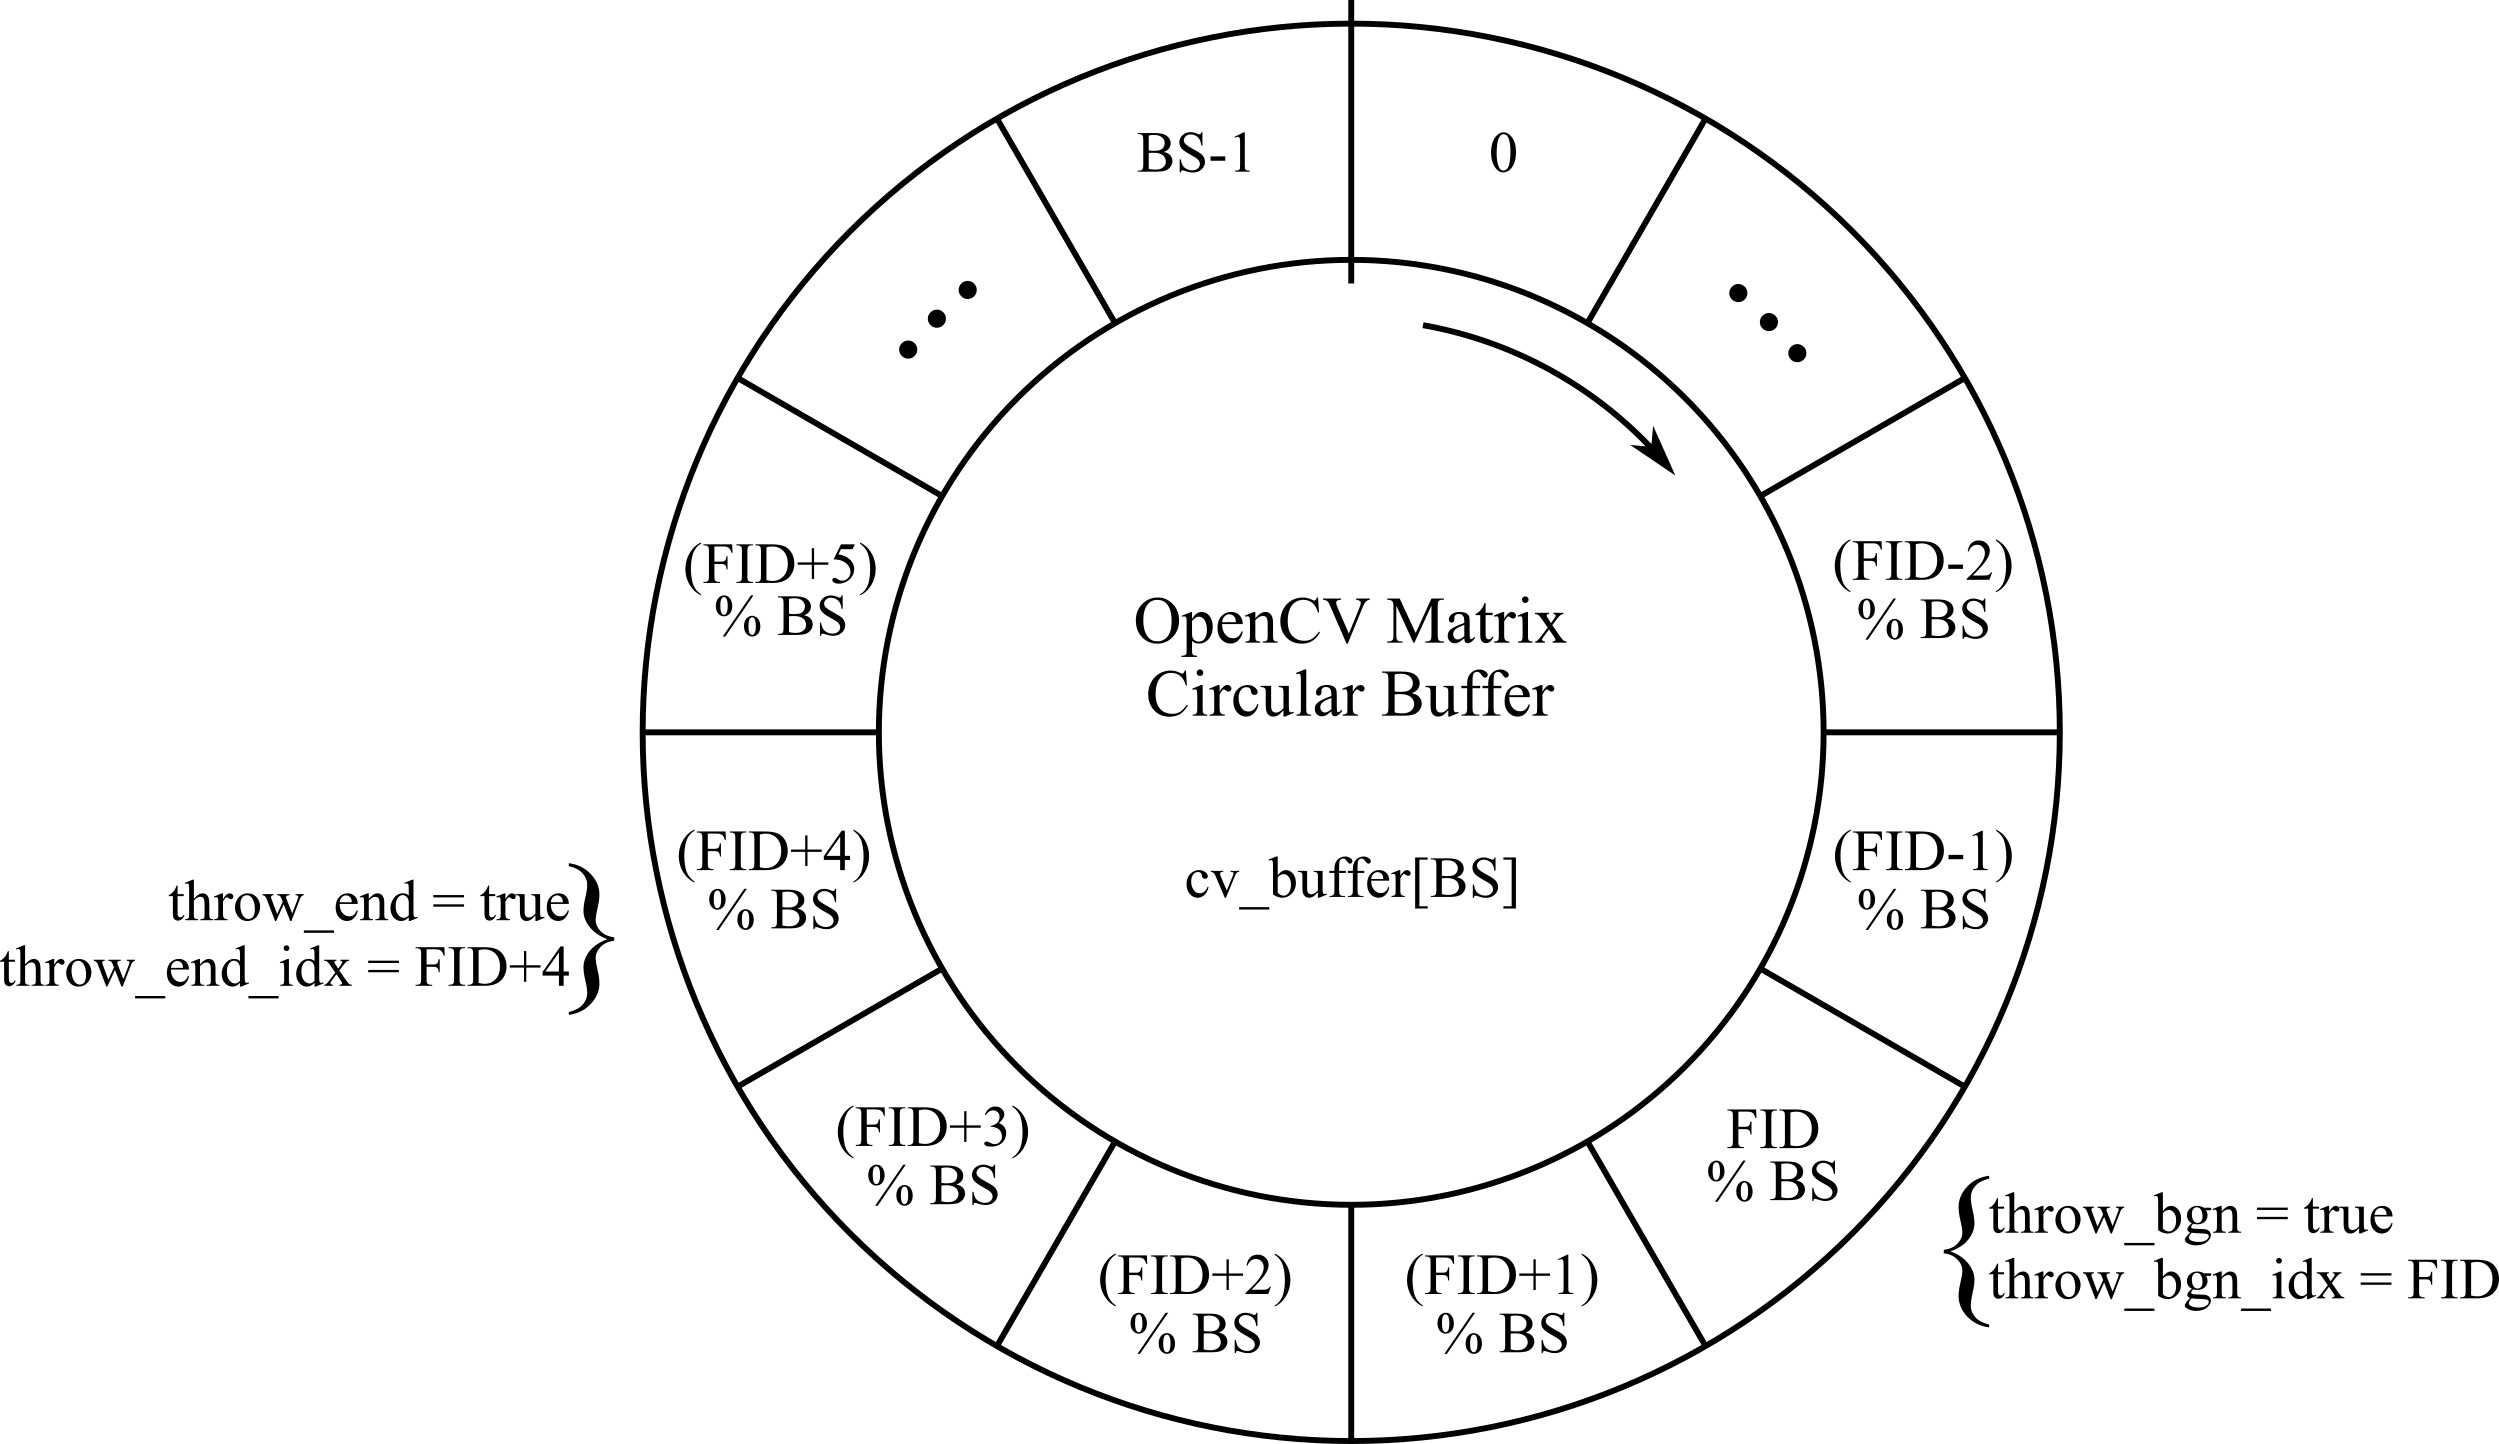
\includegraphics[width=0.9\textwidth]{buffer}
  \caption{OpenCV matrix circular buffer}
  \label{fig:circular_buffer}
\end{figure}

\subsubsection{Image Change Detection}
\label{subsubsec:image_change_detection}

This section describes the implementation of the image change detection.
The difference computation and the averaging among all the pixels is done for every frame except the first one ($\texttt{FID} \geq 1$).
The threshold comparison and the throw detection is done for every frame after the threshold has been determined (see section \ref{subsubsec:threshold}).

% --------------------------------
\paragraph{Difference Computation}
The absolute difference pixel matrix $D$ can be calculated using equation \ref{eq:abs_diff}.
The implementation uses the OpenCV function \texttt{cv::absdiff} to calculate the per-element absolute difference between the two pixel matrices and saves it into \texttt{cv\_abs}, as shown in appendix \ref{app:throw_detection} on line \ref{lst:ln:abs_diff} \cite{opencv_ooa_absdiff}.

\begin{equation}
  D = |I_\text{FID} - I_\text{FID-1}| \quad\quad \text{with} \quad\quad \text{FID} \geq 1
  \label{eq:abs_diff}
\end{equation}

\begin{tabular}{rl}
  $D =$ & absolute difference pixel matrix \\
  $I =$ & image pixel matrix \\
\end{tabular}
\\

% --------------------------------------
\paragraph{Average among all the pixels}
The mean absolute difference $\overline{\text{MD}}$ can be calculated using equation \ref{eq:mean_diff}.
The implementation uses the OpenCV function \texttt{cv::sum} to return the sum of array elements for each channel independently, as shown in appendix \ref{app:throw_detection} on line \ref{lst:ln:mean_diff}.
Since the Baumer \texttt{BayerRG8} pixel format consists of only one channel, the zeroth element is used \cite{opencv_ooa_sum}.

\begin{equation}
  \overline{\text{MD}} = \frac{1}{w\cdot h} \cdot \sum\limits_{i=1}^h \sum\limits_{j=1}^w D_{i,j}
  \label{eq:mean_diff}
\end{equation}

\begin{tabular}{rl}
  $\text{MD} =$ & mean absolute difference \\
  $D =$ & absolute difference pixel matrix \\
  $w =$ & width of the image in px \\
  $h =$ & height of the image in px \\
\end{tabular}
\\

% --------------------------------------------------
\paragraph{Threshold Comparison and Throw Detection}
Listing \ref{lst:throw_detection} shows the implementaion of the threshold comparison and the throw detection.
Due to the specific implementation, it is possible to detect a single frame change.
This means that the image changes between two consecutive frames and then stays the way it is (e.g. sudden change of the ambient light).
Such a glitch is not a valid throw and shall therefore be ignored (see line \ref{lst:ln:glitch_removal}).
Figure \ref{subfig:algorithm_example_1} shows that a valid throw of an object would create at least two changes between individual frames.
The first one by entering and the second one by leaving the frame.

As long as no throw is detected, the current Baumer \texttt{Buffer} object is released after each processed frame (see listing \ref{lst:buffer_release}).
Whenever a glitch is removed, the size of the Baumer image buffer (\texttt{BS}) is reduced by one.
This is due to the fact that no reference to past \texttt{Buffer} objects is kept.
Such a reference is necessary to release the respective buffer entry.
It would be easy to solve this by keeping track of at least one past \texttt{Buffer} object.
However, this is not necessary, provided that the buffer size is large enough.

\clearpage

\begin{lstlisting}[style=C++, caption={Throw detection and glitch removal}, label=lst:throw_detection]
  if (mean_diff >= threshold) {
      if (!throw_bgn) {
        throw_bgn_idx = frame_id;
        throw_bgn = true;
      }
  } else {
    if (throw_bgn) {
      throw_end_idx = frame_id;

      // Remove glitches (single frame changes)
      if ((throw_end_idx - throw_bgn_idx) == 1) {(*\label{lst:ln:glitch_removal}*)
        throw_bgn = false;
      } else {
        throw_end = true;
      }
    }
  }
\end{lstlisting}

% BUG: Should not be released directly but with a delay of one!
\begin{lstlisting}[style=C++, caption={Release of the filled Baumer \texttt{Buffer} object}, label=lst:buffer_release]
  if (!throw_bgn) {
    pBufferFilled->QueueBuffer();
  }
\end{lstlisting}

\subsubsection{Threshold Value Determination}
\label{subsubsec:threshold}
% \todo[inline]{Citations, Nico is this correct (regarding the 50 Hz flicker)?}

% how is the Threshold Value Determination done:
% average difference to obtain threshold (with pictures)
    % => 50 Hz flicker reduction

\begin{figure}[H]
  \centering
  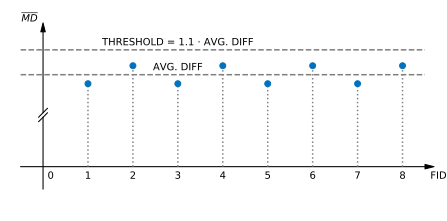
\includegraphics[width=0.75\textwidth]{threshold}
  \caption{Derivation of the threshold value from eigth averaged differences} % 
  \label{fig:threshold}
\end{figure}

\subsubsection{Saving Images}
\label{subsubsec:saving_images}
% \todo[inline]{Citations, Why PNG and not BMP or JPG?}

Resulting in the file names `\texttt{$\{0..(N-1)\}$.png}' (with $N$ beeing the amount of valid frames).

\begin{lstlisting}[style=C++]
  for (int i = throw_bgn_idx; i < (throw_end_idx - 1); ++i) {
    cv::cvtColor(cv_buffer[i % buff_size], cv_transformed, cv::COLOR_BayerBG2BGR);
    cv::imwrite(output_path + std::to_string(i - throw_bgn_idx) + ".png", cv_transformed);
  }
\end{lstlisting}

% https://www.baumer.com/ch/en/service-support/know-how/technical-information-industrial-cameras/baumer-gapi-and-opencv/a/baumer-gapi-and-opencv

